\chapter{Evaluation}
\label{evaluation}
In previous chapters detailed working of the planning algorithm has been discussed, this chapter discusses the evaluation criteria and results in detail. Various concepts discussed previously will be examined here through a series of experiments reflecting real-life driving scenarios. This chapter is organised as follows: Section \ref{experiments} discusses the systematic evaluation of the planner by exposing it to various situations equivalent to on-road driving conditions. The next section \ref{criteria_based_eval} discusses a criteria-based assessment for the planner by examining factors such as feasibility, optimality, completeness, run-time etc.

\section{Experiments}\label{experiments}
Due to time and resource constraint, most of the experiments to evaluate the planner are performed on the simulator. The test cases involve finding a collision-free path with obstruction in driving lane, avoiding slow moving traffic, merging into ongoing traffic, lane changes etc. The following subsections detail further about each experiment. 

\subsection{Lane blocked}
The scenario presented in \ref{lane_blocked_1} describes a situation when the driving lane is blocked by a static obstacle, and there is a vehicle driving in next lane. The ego vehicle slows down till the left lane is free, overtakes the slow-moving obstacle and shifts back to original lane and drives at increased speed. 

\begin{figure}[h]
    \centering
    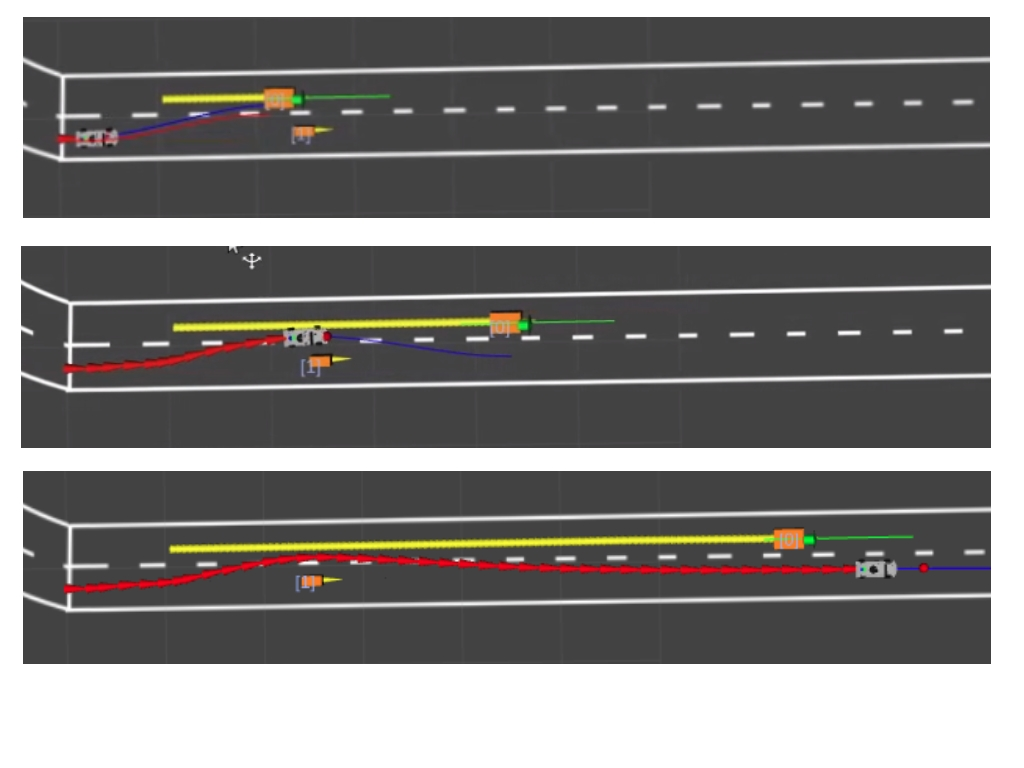
\includegraphics[width=0.7\textwidth]{Images/evaluation/2_lane_blocked.jpg}
    \caption{Driving Lane is blocked by a static obstacle with an obstacle moving in next lane. The ego vehicle avoids the static obstacle by driving into next lane and comes back to intended lane once it is free}
    \label{lane_blocked_1}
\end{figure}

\subsection{Overtaking and Merging into Traffic}

Overtaking slow moving obstacles and merging into traffic are two scenarios which are always encountered by the vehicles during on-road driving. The planner proposed in this thesis is capable of performing these two behaviours to enable autonomous driving. 

In the scenario presented in Figure \ref{slow_moving_1}, there are two slow-moving obstacles ahead of the ego vehicle. Initially, ego-vehicle picks up the speed but does not change lane as staying in the same lane is prioritised over accelerating higher. Once ego vehicle is close to the obstacle, it has to brake or shift lane, as shifting lane is prioritized over braking ego vehicle shifts into the left lane and starts accelerating. The velocity of obstacles is $0.3ms^{-1}$. 

\begin{figure}
	\centering
	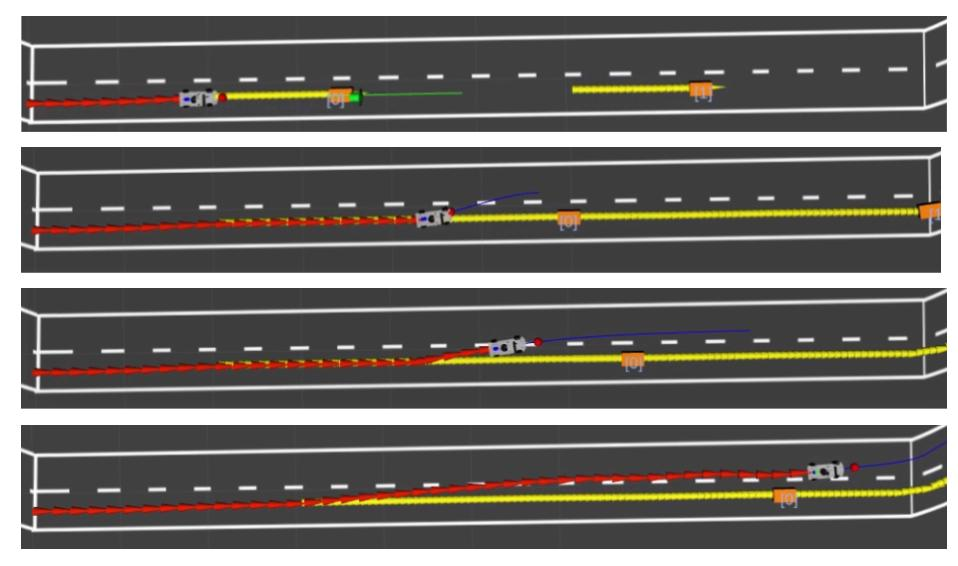
\includegraphics[width=0.8\textwidth]{Images/evaluation/overtake_1.jpg}
	\caption{Ego vehicle initially picks up the speed, when the obstacle is in collision range ego vehicle starts shifting into left lane and overtakes the slow moving obstacle}
	\label{slow_moving_1}
\end{figure}


Another general behaviour encountered by vehicles during on-road driving is merging between two obstacles. In the situation presented before, once the ego overtakes first slow-moving obstacle, it can either merge into the gap between the two obstacles as presented in Figure \ref{merging_1} or follow the left lane until the second obstacle is cleared as presented in Figure \ref{no_merge}. The cost functions are tuned such that driving in intended lane (provided by behavioural layer) is preferred over accelerating, acceleration or driving in non-intended lane is preferred over decelerating. These cost functions create behaviours of merging or non-merging. The Figure \ref{time_vel} presents velocity change over time for the behaviour of overtaking and merging into the left intended lane. Though the planner produces smooth velocity trajectories as presented in Figure \ref{velocities}, due to limitations in controller and platform the final behaviour is not smooth.

\begin{figure}
	\centering
	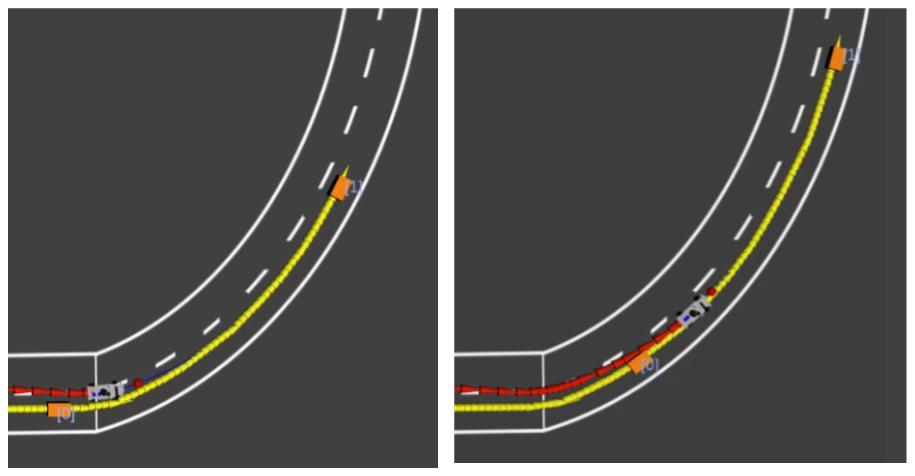
\includegraphics[width=0.8\textwidth]{Images/evaluation/merging_1.jpg}
	\caption{After overtaking first obstacle as mentioned in \ref{slow_moving_1}, ego vehicle merges into right lane between two vehicles.}
	\label{merging_1}
\end{figure}

\begin{figure}
	\centering
	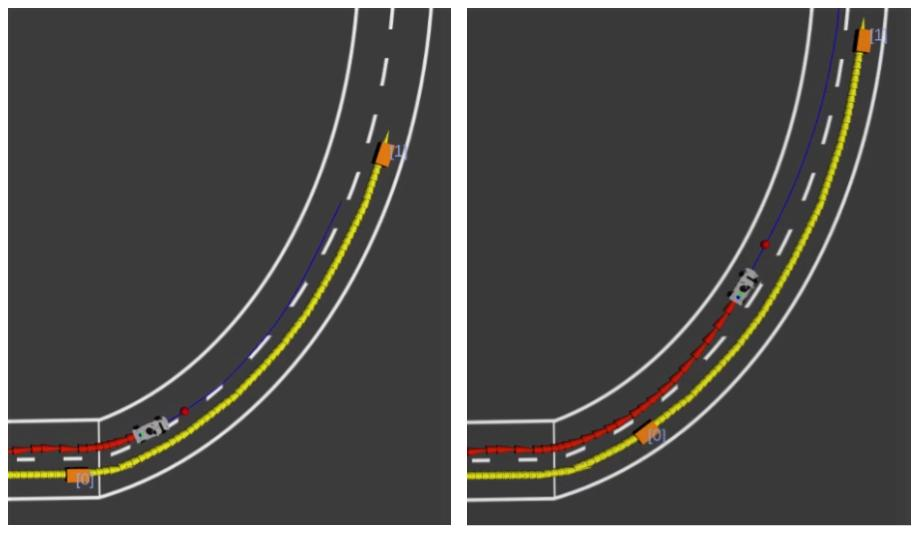
\includegraphics[width=0.8\textwidth]{Images/evaluation/no_merging.jpg}
	\caption{After overtaking first obstacle as mentioned in \ref{slow_moving_1}, ego vehicle does not merge into right lane and continues in left lane.}
	\label{no_merge}
\end{figure}


\begin{figure}
	\centering
	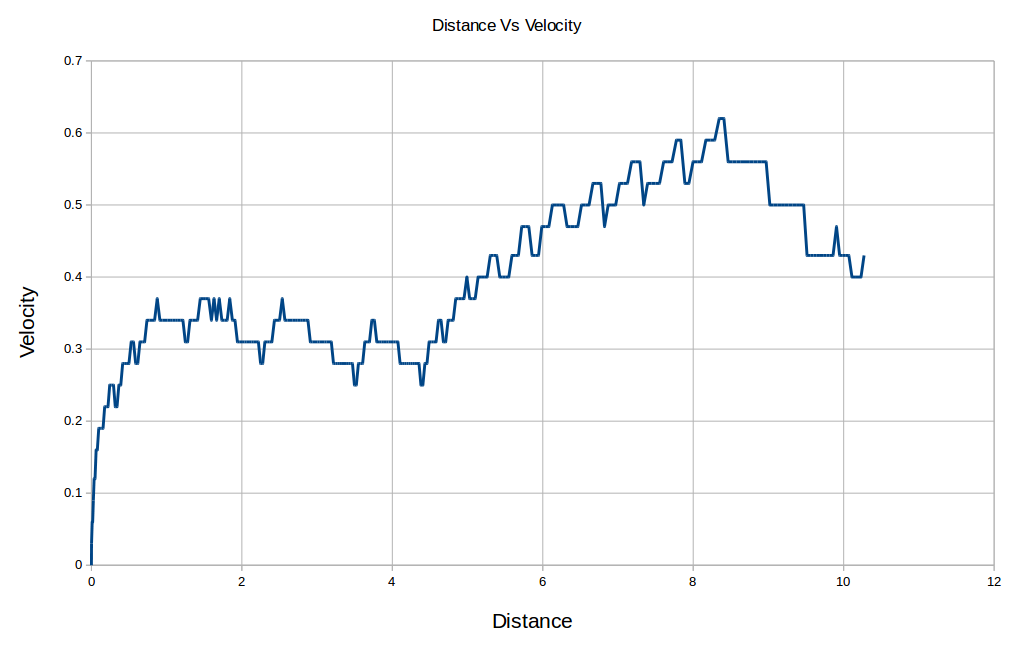
\includegraphics[width=0.8\textwidth]{Images/evaluation/overtaking_dist_vel.png}
	\caption{Velocity variation of ego vehicle with respect to time for overtaking and merging back into right lane, figures \ref{slow_moving_1}, \ref{merging_1} indicate behavior of car on track.}
	\label{time_vel}
\end{figure}



\iffalse 

In situation one presented in Figure \ref{slow_moving_1} ego vehicle starts changing into left lane once a slow-moving obstacle is encountered, once the obstacle is passed it starts driving into right lane again. In situation two presented in Figure \ref{slow_moving_2} there are two slow-moving obstacles ahead, once the ego vehicle overtakes the initial obstacle it shifts to the first lane as intended but it encounters the second slow-moving obstacle and shifts to left lane again. This behaviour is caused because of locally optimal cost functions driving the ego vehicle into the intended lane without knowledge of long-term planning information. A behavioural layer with longer scenario analysis horizon will result in better path selection.


\begin{figure}[h]
    \centering
    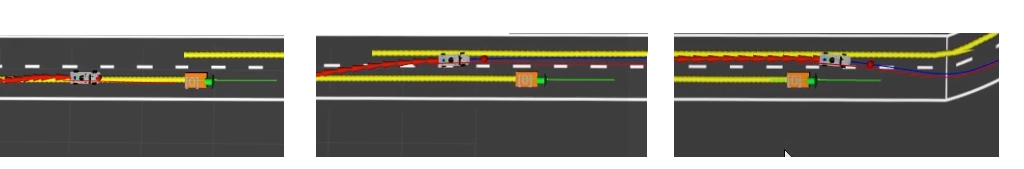
\includegraphics[width=0.8\textwidth]{Images/evaluation/slow_moving1.jpg}
    \caption{Slow Moving Traffic Situation 1}
    \label{slow_moving_1}
\end{figure}

\begin{figure}[h]
    \centering
    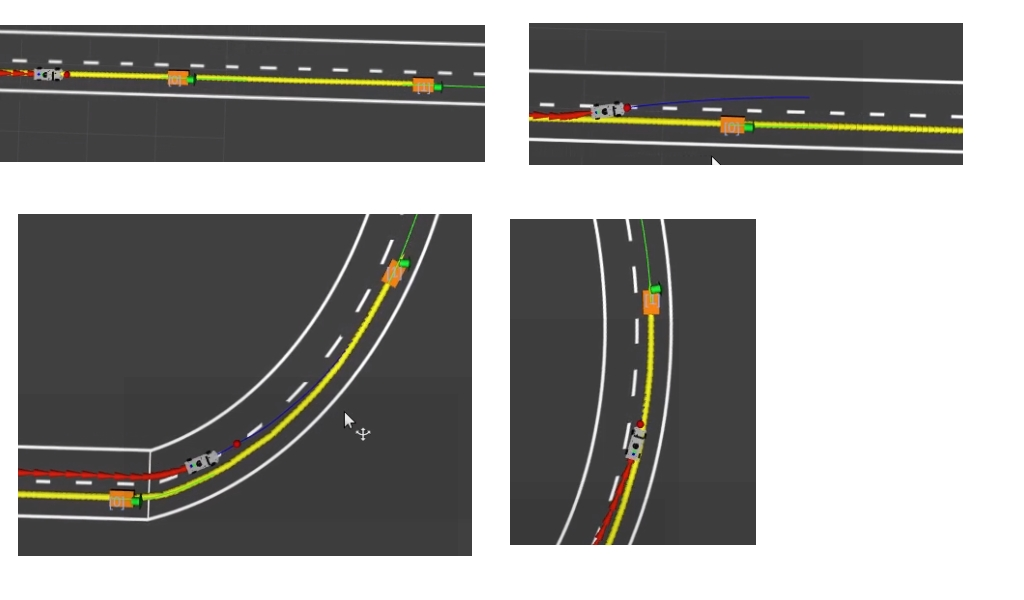
\includegraphics[width=0.8\textwidth]{Images/evaluation/slow_moving2.jpg}
    \caption{Slow Moving Traffic Situation 2}
    \label{slow_moving_2}
\end{figure}



\subsection{Merging into traffic}

In the scenario presented in Figure \ref{merging1}, lane changing is requested to merge into the traffic in the left lane. Here ego vehicle speed is $1ms^{-1}$ and obstacle speed is $0.6m^{-1}$. Initially, lane change does not occur as cost functions are tuned to maintain speed over maintaining required lane. As the vehicle enters the curve, target driving speed is reduced, and the vehicle merges into the traffic in the left lane. Depending on which portion of the lane the ego vehicle is in, i.e., near intersections or exits target lane should have higher priority over maintaining speed and during rest of the regions target speed should be of higher priority to reach a destination quickly. Cost functions implemented in this thesis provide flexibility in tuning behaviour of the ego vehicle. 

\begin{figure}[h]
    \centering
    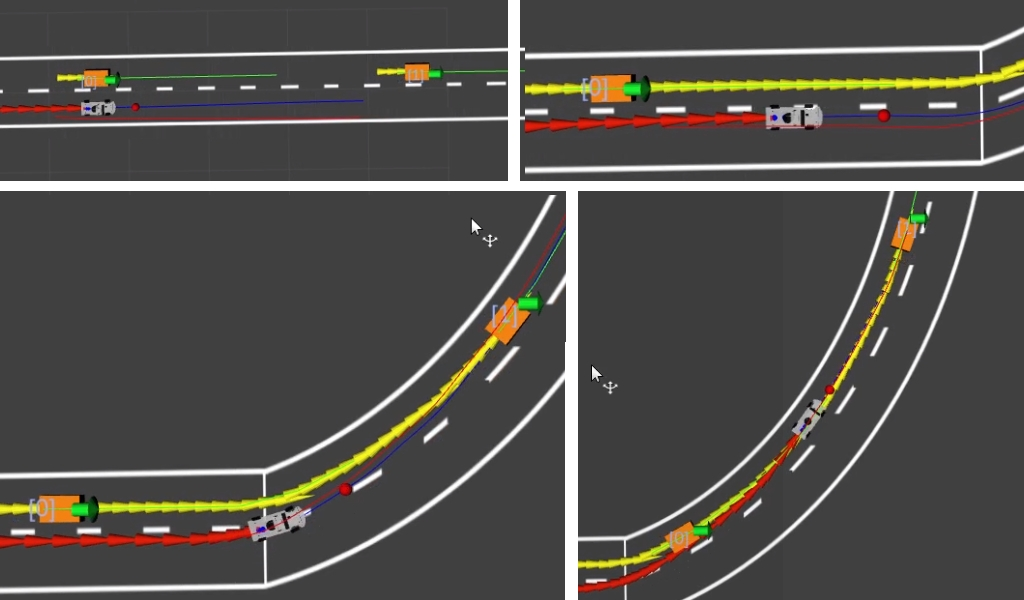
\includegraphics[width=0.8\textwidth]{Images/evaluation/merging1.jpg}
    \caption{Merging into Traffic}
    \label{merging1}
\end{figure}

\fi

\subsection{Merging into next lane with opposite traffic}

In the scenario presented in Figure \ref{series_obstacles} driving lane is blocked by a series of obstacles and the left lane is occupied by a moving obstacle. Ego vehicle starts slowly in the driving lane and waits till the obstacle is passed in the left lane and starts driving forward. 
\begin{figure}
    \centering
    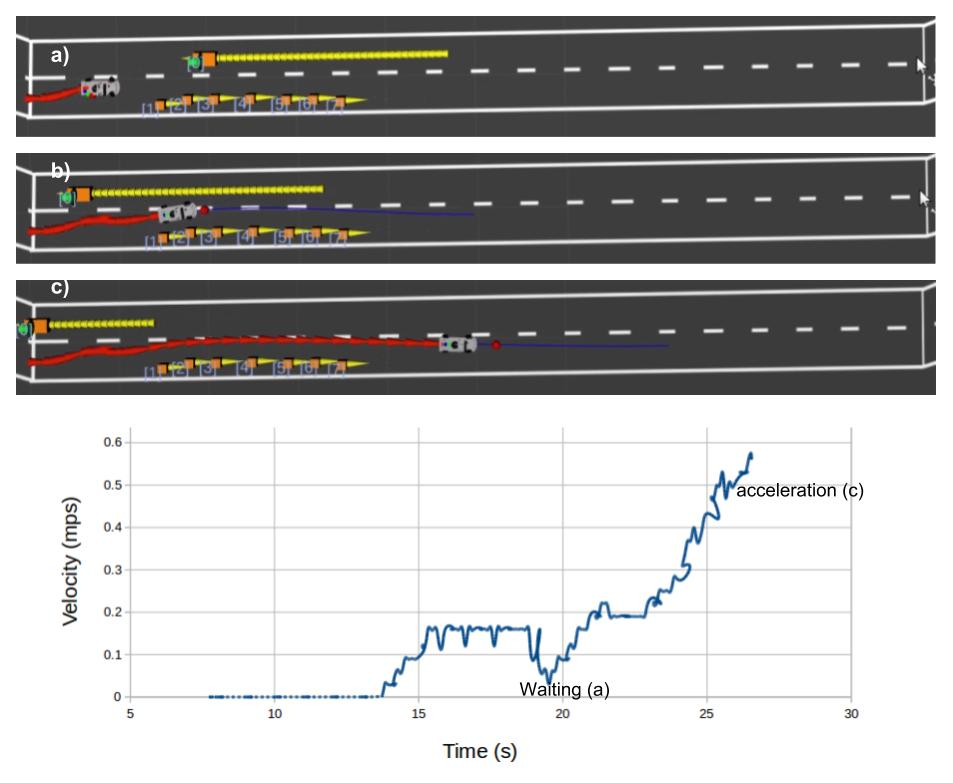
\includegraphics[width=1.0\textwidth]{Images/evaluation/vehicle_opp_1.jpg}
    \caption{Lane blocked by series of static obstacles and vehicle in next lane driving opposite. Ego vehicle waits for the vehicle to pass then drives ahead avoiding the static obstacles. The time vs Velocity charts shows how the ego vehicle starts driving, then waits for obstacle to pass and continues accelerating further after passing obstacles.}
    \label{series_obstacles}
\end{figure}

In the scenario presented in Figure \ref{series_obstacles_2}, ego vehicle has enough slack to avoid the series of static obstacles and get back into the right lane avoiding a collision with the dynamic obstacle ahead. 

\begin{figure}
	\centering
	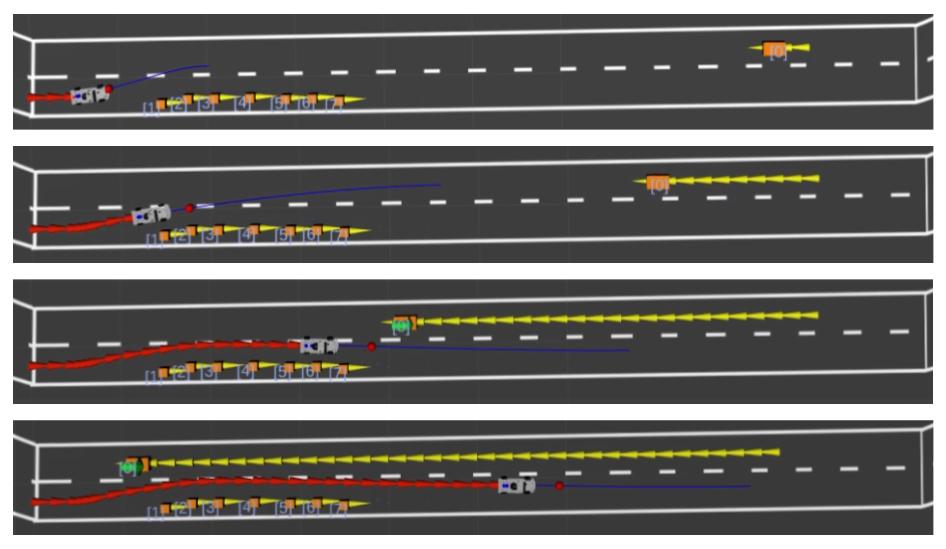
\includegraphics[width=1.0\textwidth]{Images/evaluation/vehicle_opp_2.jpg}
	\caption{Obstacle is far away on the opposite lane, ego vehicle gets enough time to overtake the obstacles and shift into right lane.}
	\label{series_obstacles_2}
\end{figure}

The ego vehicle may get stuck in the middle of the road if driving speed of ego vehicle is low, because of short temporal horizon it may not see the fast moving dynamic obstacle faraway and change the lanes. Once it's in opposite lane and sees a fast moving obstacle, ego will not to shift to right lane because of obstacles and will stop. Only if the opposite vehicle stops and provides enough slack ego will be able to drive forward. The planner does not allow reverse driving thus the ego has to switch to a different planner if the ego has to drive backwards in this scenario. 


\subsection{Road Blocked or Pedestrian Ahead}

In the scenario presented in Figure \ref{road_blocked}, the road is blocked by a series of static obstacles, the ego accelerates initially when obstacles are far away, then slows down and finally stops when it cannot find route ahead. 

\begin{figure}
    \centering
    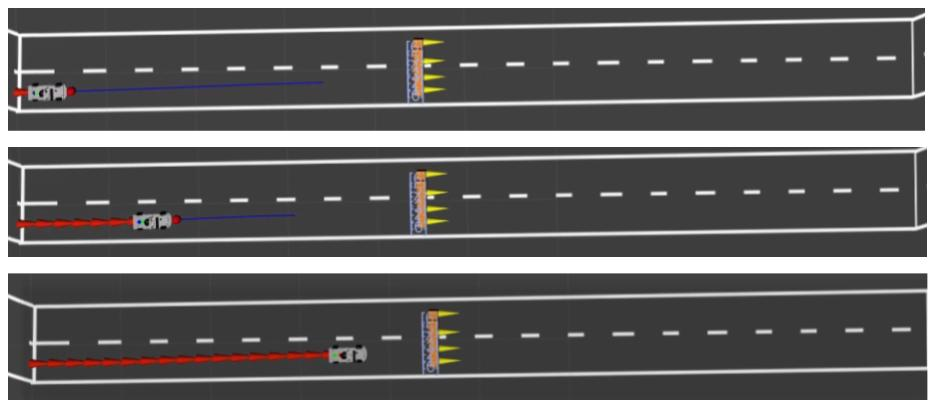
\includegraphics[width=1.0\textwidth]{Images/evaluation/stopping_lane_blocked.jpg}
    \caption{Road Blocked by series of obstacles, ego vehicle initially plans a path with acceleration, as it nears obstacles it slows down and finally stops.}
    \label{road_blocked}
\end{figure}

A pedestrian on the road is considered similar to a road blocking, in this thesis pedestrians moving across the street are set to occupy the width of the lane. In the situation as shown in Figure \ref{pedestrian_ahead} the ego vehicle initially drives at full speed, then the ego slows down (shorter blue line representing a slower speed), and the robot finally comes to a halt few meters ahead of the pedestrian. Buffer distance is a tunable parameter and currently at the maximum value for safety. 

\begin{figure}
    \centering
    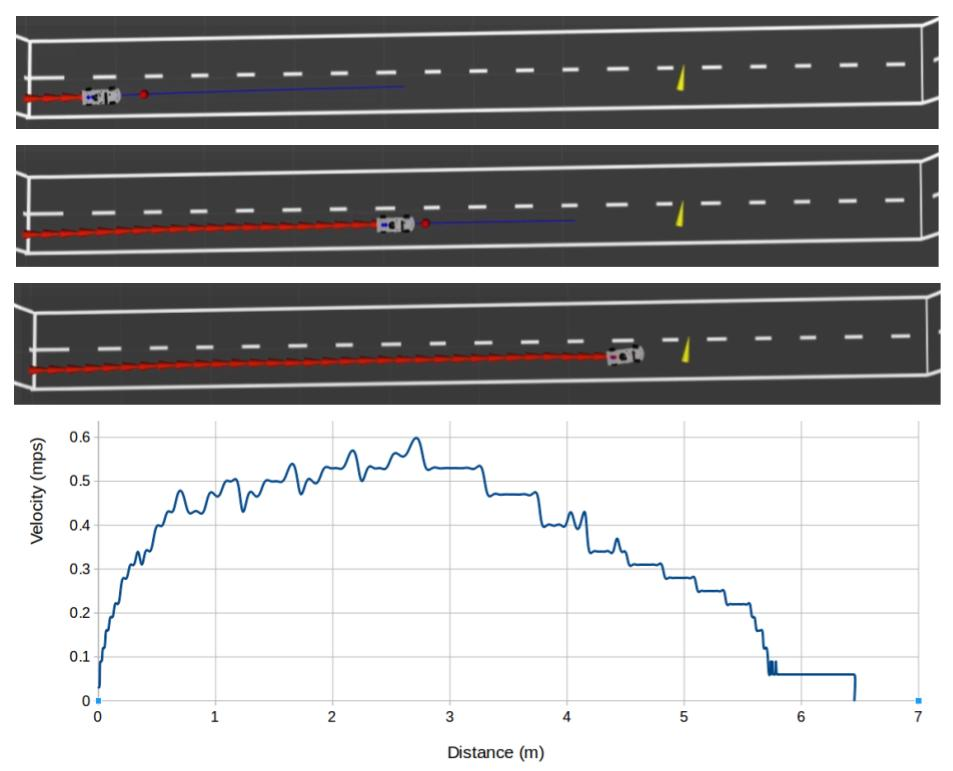
\includegraphics[width=0.8\textwidth]{Images/evaluation/stopping_pedestrian.jpg}
    \caption{Pedestrian Ahead on Road, Pedestrian is assumed to occupy lane width. Ego vehicles behaves same as lane blocked. The distance Vs velocity graph shows how the ego accelerates, then slowly decelerated and finally halts. Ego stops with 1m gap to pedestrian.}
    \label{pedestrian_ahead}
\end{figure}

\subsection{Dynamic Obstacles - other vehicles}
The main objective of the planner is to adjust to the sudden changes in the environment caused by the dynamic obstacles in surroundings, here two sub-scenarios are described where the ego vehicle has to react to an unexpected breaking of vehicles ahead. 

In the scenario presented in Figure \ref{dynamic_1}, the obstacle ahead stops suddenly, and the ego vehicle has to find a path avoiding a collision. This situation is similar to when a car ahead stops to drop off a passenger or stops for a parking spot. In this situation, ego follows the obstacle ahead, once it stops ego slows down till it finds enough room in the left lane to drive ahead of the stopped dynamic obstacle and continues driving. 

\iffalse 

\fi
\begin{figure}
    \centering
    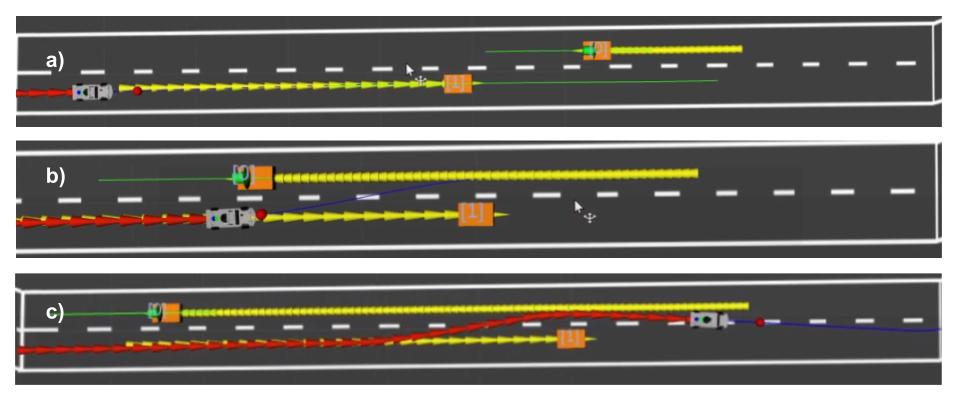
\includegraphics[width=0.8\textwidth]{Images/evaluation/sudden_Stop_dyn_1.jpg}
    \caption{The scenario has one obstacle moving along the road and other moving opposite as shown in a), ego slows down as the dynamic obstacle in the same lane stops suddenly and starts planning path in next lane once other lane is free as shown in b) and finally ego returns to original lane as presented in c) }
    \label{dynamic_1}
\end{figure}

In the scenario presented in Figure \ref{dynamic_2} two dynamic obstacles are moving ahead of the ego and threshold for safety has been chosen to be 1s. The obstacles ahead stop suddenly representing a situation of a crash for the vehicle forward or emergency stop and ego vehicle comes to a halt in next 2s. Higher deceleration profiles used in planning allow for ego vehicle to act reactively and stop without collision. 

\begin{figure}
	\centering
	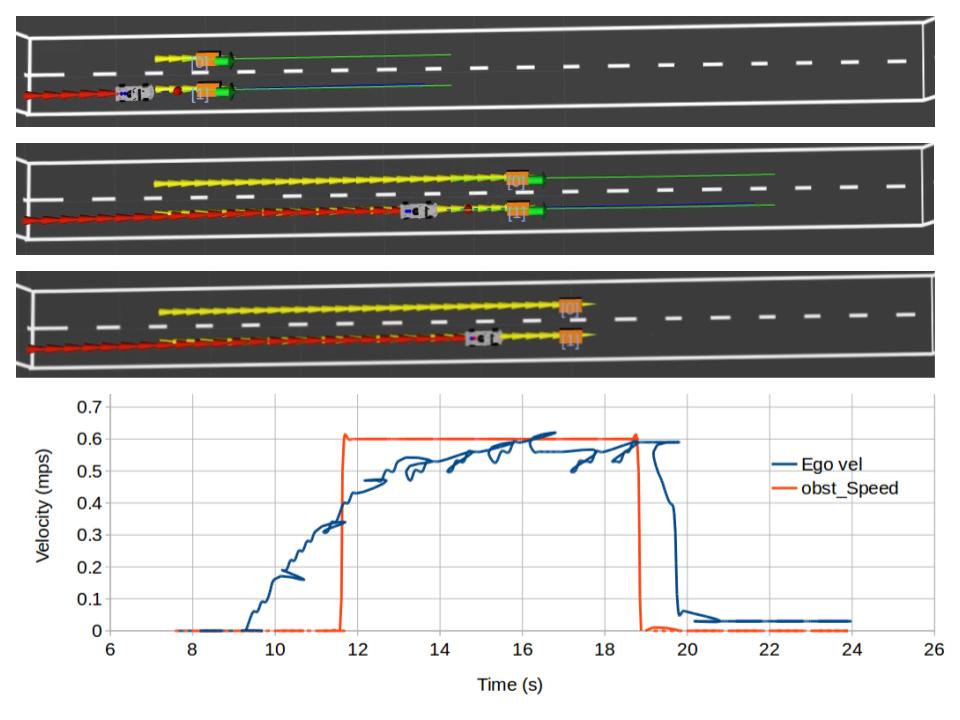
\includegraphics[width=0.8\textwidth]{Images/evaluation/sudden_stopping_lane_blocked_2.jpg}
	\caption{Ego vehicle follows two dynamic obstacles moving at $0.6ms^{-1}$ and they stop suddenly, ego vehicle decelerates quickly to stop from colliding. The chart displays velocity variation for ego vehicle with respect to obstacle speed.}
	\label{dynamic_2}
\end{figure}



 


%\subsection{Avoiding Static Obstacles}
%\subsection{Avoiding Dynamic Obstacles}
%\subsection{Avoiding Pedestrians}
%\subsection{Lane Changing}
%\subsection{Series of Static Obstacles}
%\subsection{Road Blockades}
%\subsection{Intersection}
%\subsection{Oncoming traffic}
%\subsection{Dynamic Obstacle breaking suddenly}
%\subsection{Merging into traffic to avoid other obstacles}


\section{Criteria Based Evaluation}
\label{criteria_based_eval}
In this section, the proposed planner is validated against the common criteria of evaluating any algorithm, i.e.\ optimality, feasibility, completeness, runtime and approach.

\subsection{Optimality}
 In this thesis, we discuss the optimality of the time horizon, subsection \ref{timing_constraints} already defines regarding various timing constraints chosen in this planner. A larger planning horizon will enable the planner to create a longer and better path, but due to the unpredictability of the environment, the plan created will not be valid after a specified duration, a broader horizon will also increase the run-time of the algorithm. The planner proposed in this thesis is only a local planner and always needs inputs from a behavioural layer or a global planner to choose target lane, velocity etc. thus a short planning horizon sufficient to bring the ego to a halt is suitable for the proposed planner. 

An example of how horizon will affect optimal planning for the current planner is shown in figure \ref{horizon_optimality}. Here T0, T1 are the trajectories with horizon "T" and T2, T3 are trajectories with horizon "T'". In this condition, if a lane change has been requested then trajectory T1 is chosen, but with increased horizon trajectory T3 will be selected, depending on situation one is efficient sometimes and other in others. These situations can be improved by lane selection algorithm in the behavioural layer which looks for occupancy of different lanes and suggests the one best suitable lane. Similarly, if an exit has to be taken on the road, a long horizon would choose a plan with reduced speed compared to a high-speed path with the short horizon, this can also be solved by having a velocity planner in the behavioural layer with more extended scenario analysis algorithm.  

\begin{figure}[h]
    \centering
    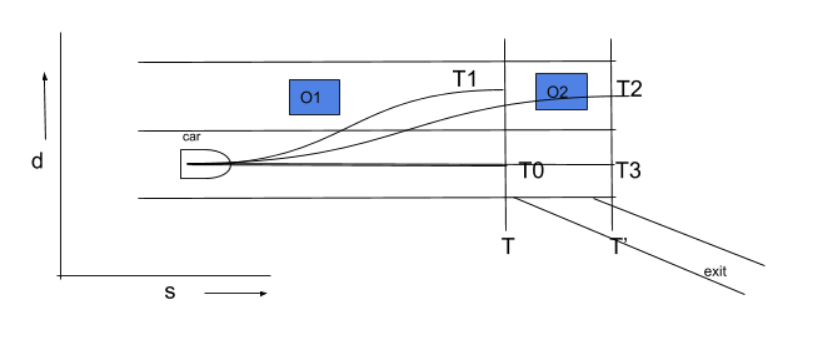
\includegraphics[width=0.8\textwidth]{Images/horizaon_optimality_2.png}
    \caption{Horizon Optimality reference}
    \label{horizon_optimality}
\end{figure}
 
 \todo{move to future works}
Another horizon generally in the discussion for a planner is spatial horizon which discusses how long is the path generated. As per the planning criteria, spatial horizon depends on velocity and temporal horizon, at low speeds spatial horizon is shorter and at high speeds larger temporal horizon. A shorter spatial horizon might result in not having a globally optimal solution, more substantial scenarios analysis will promote a local decision suitable globally. As shown in figure \ref{optimized_reference}, following the original reference path(solid line) at low speeds will result in two times collision avoidance and shifting path. With scenario analysis, a new shifted reference path can be chosen which avoids many shits improving comfort.

The resolution of the sampling in acceleration selection and lateral distance selection will also affect the optimality of planning, a chosen plan can only be optimal of the trajectories created by sampling, higher the number of samples, larger are the possibilities, and the best selection is possible. 

In summary, the planner proposed in this thesis is locally optimal and needs support from a scenario analysis algorithm to choose globally optimal paths. 
 
 \begin{figure}[h]
    \centering
    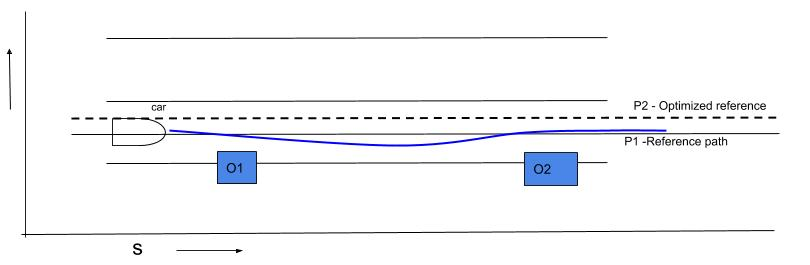
\includegraphics[width=0.8\textwidth]{Images/evaluation/optimized_reference.jpg}
    \caption{With current reference path (solid black line) at low speeds ego will follow path similar to suggested in blue curve. While with an optimised reference (dotted line) ego will move straight without many shifts}
    \label{optimized_reference}
\end{figure}

\subsection{Feasibility}
\label{feasibility}
The ability of the vehicle to traverse the created trajectory determines feasibility. Generally, the curvature of the path, smoothness and accelerations determine whether a trajectory is feasible or not. The proposed planner creates feasible trajectories at lower speeds because of the third order splines used, and higher speeds require fifth or higher order splines to maintain continuity in path curvature and speed. Discussions in \cite{cmu_parallel_thesis} \cite{ppt_teqniqs_coll_Avdnce} throw light on how to achieve higher degrees of smoothness, which approach is better in which driving conditions. As the intended application for this planner is a modelcar, constant acceleration profiles are used due to a limitation in the ability of the car to track small changes in velocity and inaccuracies in measurement. These can be easily replaced by a smoother higher order polynomial with a better hardware platform. Consistency in paths evaluated with respect to previous plan is another factor in testing feasibility, the current planner penalizes trajectories deviating from previous plan and also take into account current orientation of the vehicle in choosing a path. Thus creating smoother transitions from one state to another by respecting current driving curvature.

In summary, the planner creates feasible trajectories for the modelcar and needs  update in polynomials used in trajectory creationa and representation to be used in complete cars. 

\subsection{Completeness}
\label{completeness}
An algorithm is said to be complete if it can result in a solution every time. A motion planner can be called complete if it returns path if it exists in the space searched. Like many other sampling-based approaches the planner proposed in this thesis only probabilistically complete. That is, the probability of finding a solution approaches to one as the number of samples increases. If there are a higher number of samples in the configuration space, the higher are the chances of finding a solution. If a planner cannot find a solution within the sampled region, it forces the ego to perform an emergency braking manoeuvre. 

In Figure \ref{probablistically_complete}, there are only two sampled end states and there is no solution found by the vehicle, by increasing the number of lateral samples a solution can be easily found. In general condition of completeness can be improved in two ways, first is to sample as many points as possible and as closely as possible in the solution space. The second method is to keep on sampling until an end solution is found or timeout has been reached. The former method will reduce the computational performance while the later can be complex and expensive. The planner proposed in this thesis implements a combination of both methods, initially as many samples as possible are created and then evaluate only evaluate these samples based a pre-cost of sample till a feasible solution is found. It is recommended to achieve completeness for safety purposes in autonomous driving.


In summary, the proposed planner is probabilistically complete and current implementation with a limited number of acceleration profiles, and lateral shift samples are suitable for the modelcar, and higher sampling needs to be performed to improve completeness.  

 \begin{figure}[h]
    \centering
    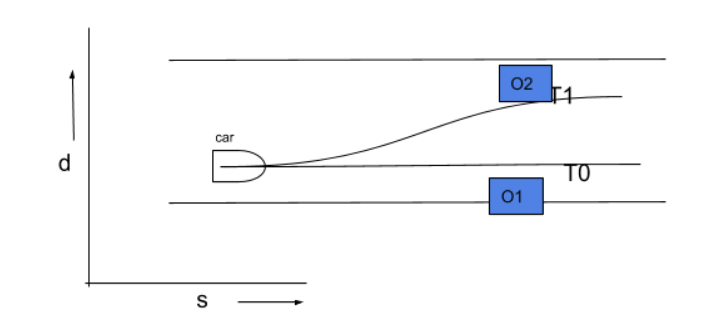
\includegraphics[width=0.8\textwidth]{Images/probablistically_complete.png}
    \caption{Probablistic Completeness}
    \label{probablistically_complete}
\end{figure}

\subsection{Runtime}

Though computation power is available cheaply, it is important to create solutions which are cheaper and can be employed in large scale. In this case, sampling based approaches perform well and run on low computational hardware. In contrast lattice-based approaches such as \cite{cmu_parallel_thesis} \cite{diss_shui_phd_thesis} \cite{werling_frenet} computationally expensive and require a GPU to run. Low computational costs mean larger chances to be adopted to a greater number of platforms.

To compute the complexity of planner lets consider $n_a$ denote the number of acceleration/deceleration profiles, $n_s$ denote the stopping deceleration profiles and $n_l$ denote the number of lateral distance samples. Then the maximum number of samples created is $(n_a+n_s)*n_l$, generally stopping profiles are less as at higher deceleration lower number of lateral samples are chosen due to limitations in vehicle dynamics. This thesis employs a hybrid combination of two methods mentioned in \ref{completeness} to achieve completeness. Therefore in the best case, only one trajectory is evaluated, and complexity is $O(1)$, and the worst case complexity is $O((n_a+n_s)*n_l)$.

Trajectory evaluation with respect to dynamic obstacles is an expensive process in the evaluation of trajectories. Simulation-based methods as discussed in  \cite{kolski_thesis} are expensive with complexity in terms of $O(n_o*n_n)$ where $n_o$ is the number of obstacles and $n_n$ is the number of simulation steps. This thesis employs a simple collision checking algorithm with constant time for evaluating one obstacle thus reducing the complexity to $O(n_o)$, number of obstacles. This process is not effective in intersections. Currently, a conservative approach to wait for other obstacles to pass is used, a simple approach as discussed in \cite{rrt_star} which has a performance better than the simulation-based algorithms can also be employed in future for intersections.  

\subsection{Deliberative Approach}
The planner proposed in this thesis maintains a mix of deliberative and reactive approach. Deliberative by evaluating a trajectory completely before committing to it, this is important to create trajectories adhering to traffic, safe and comfortable. In general, all the planners evaluate all the sampled trajectories then choose the best based on different costs. The planner proposed in this thesis does not follow this convention, and once it finds the best trajectory, it stops evaluating the other trajectories as presented in subsection \ref{traj_Selection}. It does not limit the real-time response of the trajectory as the sampling is chosen such that the worst case response time is within the hard real-time response required by the planner. 

In summary, the planner achieves a reactive behaviour with higher accelerations and trajectory selection algorithm at the same time being deliberate in selecting the final trajectory for execution. 

%\subsection{Low Computational Costs}

%Though computation power is available cheaply, it is important to create solutions which are cheaper and can be employed in large scale. In this case sampling based approaches generally fare well and run on a low computational hardware. In contrast lattice based approaches such as \cite{cmu_parallel_thesis} \cite{diss_shui_phd_thesis} \cite{werling_frenet} computationally expensive and require a GPU to run. Low computational costs can enable the technology to be adopted to a larger market. Safety should not be compromised for sake of low computational costs and the planner proposed here employs large range of acceleration profiles to bring the vehicle to halt easily in case of an emergency.

%It is true that computation is cheaper in current generation but it is important to bring down the costs to bring technology closer to larger markets. All the lattice based planners which provide the best of the performance evaluate on an average of 100,000 trajectories in one planning cycle and depend on GPUs and many multicore processing units to achieve this results. On the other hand sampling based approaches are cheaper and more conservative. The planner proposed in \cite{cmu_parallel_thesis} can perform a double lane change evasive manoeuvre equivalent to professional drivers to avoid sudden obstacles.  



%\section{Comparisons to other Planners}



%All the motion planners proposed achieve similar objective of navigating smoothly on road with different special capability, these special techniques define how and where these planners can be used. It is tough to compare the planners performance by comparing in definite scenarios due to logistical constraints and costs and objectives of different planners. The generic parameters which define the performance of a trajectory planner are deliberative evaluation, higher dimensional search space, on-road, parallel, real-time. Different types of planners proposed achieve different goals and are suitable at different conditions. 

%\subsection{Comparison to Sampling based Approaches}
%There have been many sampling based approaches that are proposed as discussed in Section \ref{related_work} for trajectory planning. One of such approach is discussed in \cite{traj_smoothing}, here the authors differentiate between the path planning and velocity planning, this approach doesn't choose a spatial or temporal horizon before thus, at high speeds it may fall short if the sampled position is shorter and at low speeds the planned path is very far into the future such that the plan is not valid anyway after some time. This un-necessarily increases the complexity. 

%\subsection{Comparison to Lattice based approaches}
%As discussed in Section \ref{related_work}, lattice based approaches are expensive computationally(generally in terms of fourth order or more based on number of dimensions in lattice), they employ lesser number of acceleration profiles as discussed in \cite{cmu_parallel_thesis} \cite{diss_shui_phd_thesis} to reduce the complexity, this could be a real problem in driving in traffic scenarios where vehicles are close to each other with not so much space for evasive manoeuvres and hard breaking is needed. Though the planner proposed in this thesis cannot create single trajectory with multiple lateral shifts to perform evasive manoeuvres like any other sampling based approach proposed, this planner employs large number of accelerations and deceleration's to improve safety. These planners are designed to run on a separate hardware such as GPU and are not suitable for low computational platforms such as modelcar. 



%Advantages of combining path and velocity? - How it can reduce sampling state. 

%Acceleration profiles for emergency stopping 

%Simulation based approaches to the proposed approach in this planner for collision checking. 

%Why it is not important to validate other trajectories once the best trajectory is found. 

%Urban driving needs strong abilities to stop immediately and lattice planners cannot do this as the number of acceleration profiles increases the evaluated trajectories gets increased in thousands. 

%Eg: CMU - increasing one acceleration will add 13000+ more trajectories, discretizing time by one more step will add 200,000 thousand more trajectories to evaluate thus limit the spatial and temporal horizon the planner can evaluate. At high speeds a larger spatial horizon is needed but generally temporal horizon remains same at all the speeds thus we chose to plan in a temporal horizon to allow planning at all multiple speeds. 


%Divide the trajectory planning and behaviour layer, with this the complexity of solving the task can be reduced drastically. If the trajectory planner need not worry about the behaviours and focus solely on driving safely it will enhance the performance of the vehicle and achieve the costs at a low computational cost.  



